\documentclass[11pt]{article}
%% Package imports
\usepackage[utf8]{inputenc}
\usepackage{amsmath}
\usepackage{subcaption}
\usepackage{amsfonts}
\usepackage{amssymb}
\usepackage{physics}
\usepackage{graphicx}
\usepackage[left=2cm,right=2cm,top=2cm,bottom=2cm]{geometry}
\usepackage{multirow}
\usepackage{booktabs}
\usepackage{siunitx}
\usepackage{float}
\usepackage{verbatim}
\usepackage{amsthm}
\usepackage{minted}
\usepackage{fancyhdr}
\usepackage[dvipsnames]{xcolor}
\usepackage{parskip}
\usepackage{minted}
\usepackage{newunicodechar}
\usepackage{blindtext}
\usepackage{hyperref}
\usepackage{titling}
\renewcommand{\baselinestretch}{1.5}

%% Commands for inserting big braces.
\newcommand\lb{\left\lbrace}
\newcommand\rb{\right\rbrace}

%% Commands for set such that notation
\newcommand\st{\text{ } | \text{ }}

\usepackage[shortlabels]{enumitem}
\setlength{\droptitle}{-7em}
\newtheorem*{theorem}{Theorem}
\renewcommand\qedsymbol{$\blacksquare$}

%% Page style settings
\pagestyle{fancy}
\fancyfoot{}
\fancyhead[L]{\slshape{Microarchitecture Optimisation in Splay Trees}}
\fancyhead[R]{\slshape{Szymon Kubica, CID: 01871147}}
\fancyfoot[C]{\thepage}
\begin{document}
\title{Coursework 1: Microarchitecture Optimisation in Splay Trees}
\date{\today}
\author{Szymon Kubica, CID: 01871147}
\maketitle

\vspace{-1em}
\section*{Studying microarchitecture effects}
\vspace{-1em}
\subsection*{Varying the size of RUU }
\vspace{-0.5em}

The figures below show the instructions per cycle and the estimated energy
consumption metrics when running the \texttt{splaytest} program as the number
of slots in the register update unit varies from 2 to 256. The datapoints are
interpolated linearly to give a better idea of the trend as the test parameter
is changed.

\vspace{-1em}
\begin{figure}[H]
  \centering
  \begin{subfigure}{.5\textwidth}
    \centering
    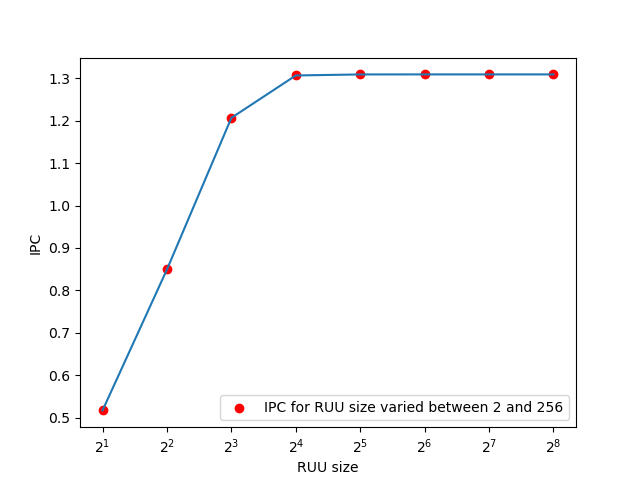
\includegraphics[width=1.0\textwidth]{"../plots/vary-ruu-ipc.png"}
    \caption{IPC for RUU sizes between 2 and 256}
    \label{fig:sub1}
  \end{subfigure}%
  \begin{subfigure}{.5\textwidth}
    \centering
    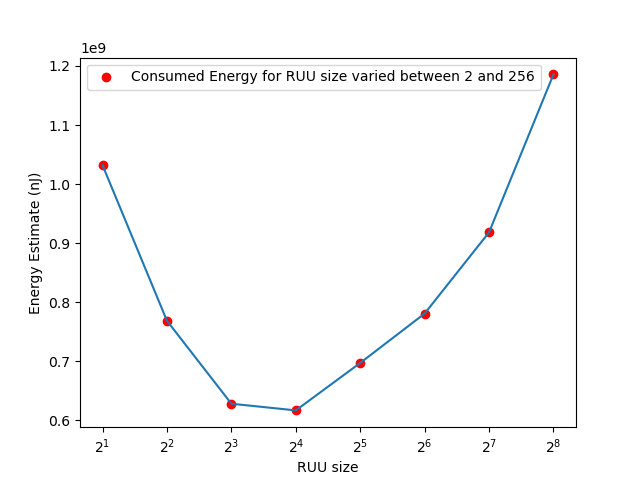
\includegraphics[width=1.0\textwidth]{"../plots/vary-ruu-energy.png"}
    \caption{Energy estimate (nJ) for RUU sizes between 2 and 256}
    \label{fig:sub2}
  \end{subfigure}
\end{figure}
\vspace{-1em}

We may observe that total energy consumption initially decreases, reaches a
minimum when the size of RUU is 16 and then starts to rise again. That's
because, when the size of RUU is 2, the simulated architecture cannot benefit
from the out-of-order execution that the RUU is supposed to facilitate. We can
see that reflected in the total IPC in that case being less than 1 for RUU
sizes of 2 and 4. After we increase the number of slots in the RUU, even though
we are using a more power-hungry RUU unit, the total energy consumption starts
to decrease. This is because  the overall IPC increases, consequently the
processor is able to execute the program within a lower execution time which
leads to a lower total energy consumption. However past the point of 16 slots
in the RUU, the performance in terms of IPC no longer increases and we are only
paying the penalty of using a more energy-hungry RUU.

\vspace{-1em}
\subsection*{Varying sizes of RUU and LSQ}
\vspace{-0.5em}
The IPC and energy consumption estimates for pairs of RUU and LSQ sizes in the
set $\lbrace 8, 16, \ldots, 256 \rbrace$ can be seen below. The graphs have been
interpolated with a triangular surface to make it easier to visualise the trend
that the data follows as we vary the parameters.
\vspace{-2em}
\begin{figure}[H]
  \centering
  \begin{subfigure}{.5\textwidth}
    \centering
    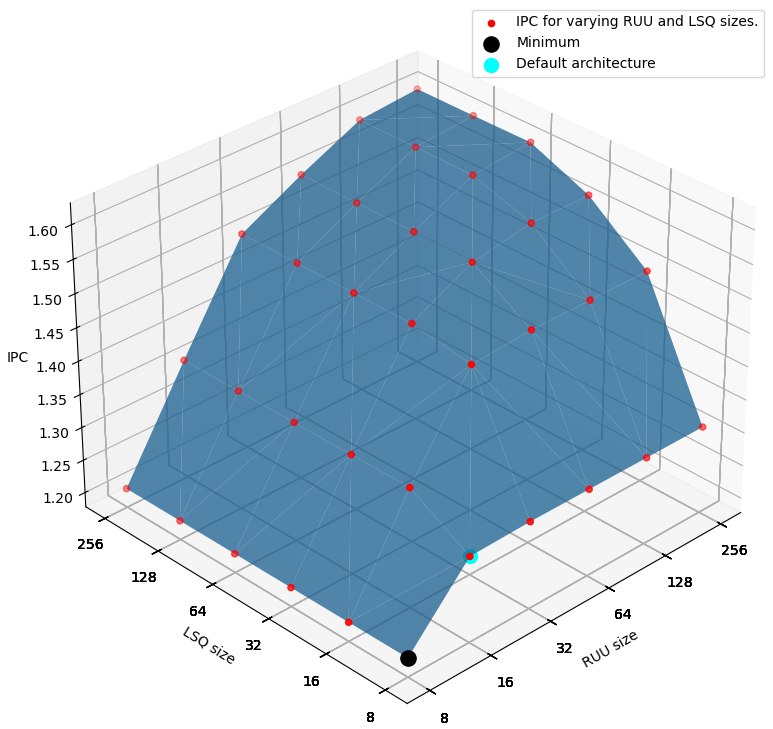
\includegraphics[width=1.0\textwidth]{"../plots/vary-ruu-lsq-3d-ipc-good-angle.png"}
    \caption{IPC for RUU and LSQ ranging 8 - 256}
    \label{fig:sub1}
  \end{subfigure}%
  \begin{subfigure}{.5\textwidth}
    \centering
    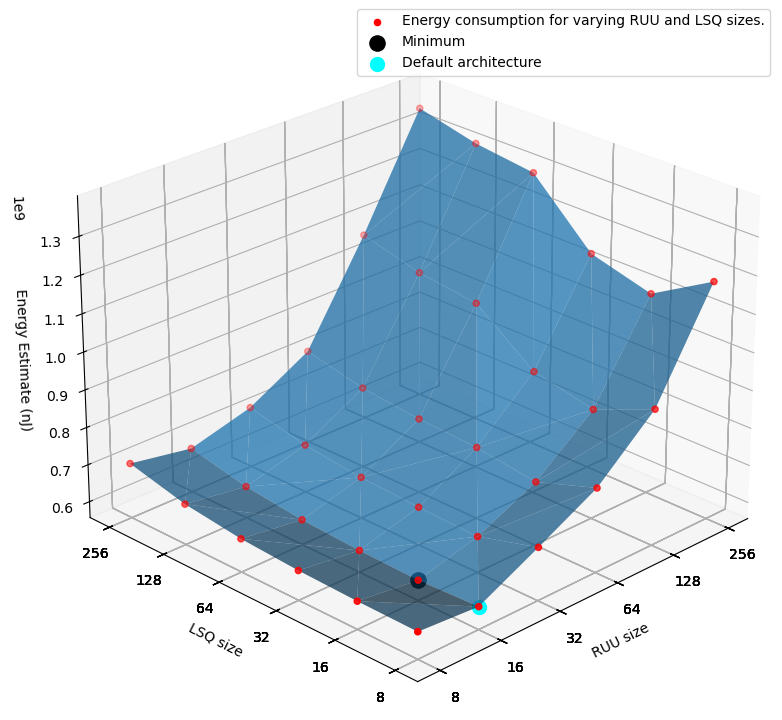
\includegraphics[width=1.0\textwidth]{"../plots/vary-ruu-lsq-3d-energy-good-angle.png"}
    \caption{Energy estimate for RUU and LSQ ranging 8 - 256}
    \label{fig:sub2}
  \end{subfigure}
\end{figure}
\vspace{-1em}

Interestingly, the figure (b) shows that as we increase the size of RUU, the
energy consumption increases rapidly, whereas the same increase in the size of
LSQ results only in a slight increase in the energy consumption. This is due to
the difference in the internal structure of the those units. The circuit of RUU
is more complicated and interacts with a larger number of components, thus
using more energy.

\vspace{-1em}
\subsection*{Bottleneck in the default simulated architecture}
\vspace{-0.5em}

The default architecture sets the RUU and LSQ sizes to 16 and 8 slots
respectively. This configuration is indicated with the cyan dot above. Figure
(a) shows that the bottleneck is caused by the interaction between those two
parameters. If we were keep LSQ size constant at 8 and only increase the of
RUU, we IPC wouldn't increase past the bottleneck point of about 1.30. The same
holds if we increased LSQ size without changing the RUU size. This is due to
the purpose of those two units, the larger the RUU allows us to have more
'in-flight' instructions in the out-of-order execution. However as the number
of those instructions increases, we need the LSQ to ensure that loads and
stores are handled correctly (other instructions depending on their data might
need access to it before it is committed to the main memory). The problem
arises when there is a big difference in size between those two units. When LSQ
is a lot larger, we aren't able to get enough in-flight instructions to utilise
all slots in the LSQ. In the other scenario we can have many instructions in
flight, however because of the small LSQ, we can't handle many repeated
loads/stores in the out-of-order execution before we need to commit the change
to the main memory. After running the \texttt{varyarch-energy-2-parameters}
script, the energy estimate was the lowest when both RUU and LSQ have 16 slots.
Note that this datapoint doesn't correspond to the lowest execution time, hence
maximising the IPC doesn't necessarily mean minimising the energy consumption.

\section*{Minimising total energy}
\vspace{-0.5em}
The figure below shows the progression of the energy estimate of the simulated
architecture as I was applying optimisations to it. The following section explains
the reasoning behind each of the seven configuration settings that I have applied
to minimise the energy consumption.

\vspace{-1em}
\begin{figure}[H]
  \centering
    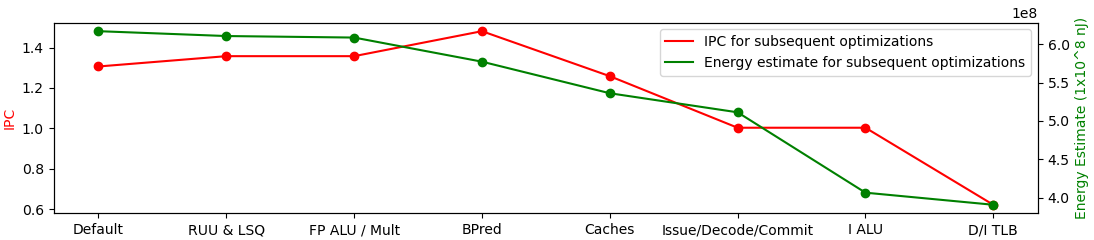
\includegraphics[width=1.0\textwidth]{"../plots/ipc-after-optimisations.png"}
    \caption{Energy Estimate and IPC for subsequent optimisations}
    \label{fig:final}
\end{figure}
\vspace{-1em}
As we previously saw, the energy estimate starting from the default
architecture is minimised when we set the size of both RUU and LSQ to 16. To
lower the energy consumption further, I set the sizes of RUU and LSQ as above
and then considered how the energy estimate is calculated. We are using
\texttt{wattch} with the \texttt{cc1} clock gating model which assumes that
each unit is fully on if any of its ports are accessed during a given clock
cycle. Because of this, I searched for parts of the microarchitecture that are
enabled by default but might be underutilised (or even not used at all). After
inspecting the code, I noticed that it doesn't perform any floating point
calculations. By default, the simplescalar simulator uses 4 floating point ALUs
and 1 fp multiplier/divider unit. I tried disabling those units entirely by
setting their number to 0, however that setting is not allowed in the
simulator. Instead, I varied the number of fp ALUs and noticed that indeed as
decreasing their number lowered the energy estimate with no impact on the IPC.

Next, I looked at the output of the \texttt{varyarch-energy-3params} script. I
noticed that the \texttt{bpred:comb} had an overall better performance and
energy efficiency across all possible configurations. Additionally, to make it
more energy-efficient, I have decreased its meta table size, and the size and
associativity its of BTB, as follows: \texttt{-bpred:comb 128 -bpred:btb 256
2}. Note that this change had a positive impact on both IPC and the energy
estimate (BPred stage in Fig. 3).


After that, I noticed that the cache miss ratio was very low. I hypothesised
that the comparatively small size of the simulated program and the small
problem size left the cache underutilised. After searching through the
parameter space of possible cache configurations, I set L1 data cache to be
direct mapped and lowered the size and associativity of the L2 data cache from
$(1024,4)$ to $(128,2)$ respectively. Interestingly, the best configuration of
the instruction L1 cache that I could find for that particular workload was a
direct mapped cache with 64 blocks of size 64 bytes with random replacement
policy (Caches in Fig. 3).

To maximise the impact on the optimisation, I decided to examine which
components use the most energy. The table below contains the \texttt{cc1} power
metrics calculated for the configuration that was found so far.

\begin{table}[H]
\begin{center}
\begin{tabular}{| l | S[table-format=12.4]| l | S[table-format=12.4]|}
  \hline
  Energy component & {Energy estimate (nJ)} & Energy component & {Energy estimate (nJ)} \\
  \hline
  \texttt{clock\_power\_cc1}   & 232728779.4305 & \texttt{issue\_stage\_power\_cc1}   & 225405153.8841 \\
  \hline
  \texttt{alu\_power\_cc1}   & 77009065.0891 & \texttt{dcache\_power\_cc1}   & 62116184.7397 \\
  \hline
  \texttt{fetch\_stage\_power\_cc1}   & 59700054.8643 & \texttt{regfile\_power\_cc1}   & 52703405.4967 \\
  \hline
  \texttt{icache\_power\_cc1}   & 46871946.9971 & \texttt{window\_power\_cc1}   & 39979548.9591 \\
  \hline
  \texttt{resultbus\_power\_cc1}   & 38483018.5632 & \texttt{bpred\_power\_cc1}   & 12828107.8673 \\
  \hline
  \texttt{lsq\_power\_cc1}   & 7791801.5251 & \texttt{dispatch\_stage\_power\_cc1}   & 6585633.4845 \\
  \hline
  \texttt{rename\_power\_cc1}   & 6585633.4845 & \texttt{dcache2\_power\_cc1}   & 25535.0078 \\
  \hline
\end{tabular}
\end{center}
\caption{Power metrics of microarchitecture components}
\end{table}
\vspace{-2em}

One can observe that a lot of energy was spent on the issue stage
(\texttt{issue\_stage\_power\_cc1}). Because of this I decided to look at
possible configurations of the issue, decode and commit stage widths
(\texttt{issue:width}, \texttt{decode:width}, \texttt{commit:width}). The
reason I was changing those in conjunction was that if we increased one of them
(e.g. \texttt{issue:width}) while keeping the remaining ones constant, we could
face a bottleneck (e.g. decode stage won't be able to process all issued
instructions as it has a lower bandwidth) Because of this I tested various
possible configurations of that triple. Interestingly, I found that the most
energy-efficient configuration was:
\texttt{(issue:width=2,decode:width=2,commit:width=8)}. I was surprised that
the commit width was comparatively larger than the other ones. A possible
reason for this could be that given that we have 16 slots in the RUU, we might
have a lot of instructions in-flight. Thus it could happen that there are more
than 2 instructions ready to commit at the end of one cycle. In which case,
having a larger commit stage as would allow for clearing the RUU more
efficiently.

Lastly, I decided to  decrease the number of integer ALU units and the size and
associativity of the TLBs. I noticed that \texttt{alu\_power\_cc1} was the
third most energy-hungry component in the architecture. In case of TLBs, I
observed that there were almost none TLB misses in the default configuration,
which might suggest that some TLB capacity wasn't utilised by the program.
Interestingly, changing the number of integer ALUs units didn't have a large
impact on the IPC, whereas it has lowered the energy estimate substantially. By
contract, by restricting the size and assoc. of TLBs, the energy efficiency
gain is relatively small compared to the massive penalty that we get in terms
of the IPC. One could evaluate if it is worth paying such a high price in terms
of performance to gain a slight improvement in the energy efficiency. To
conclude, the final energy estimate achieved was 390815492.3505 nJ which is
about 37\% decrease compared to the initial energy consumption of
616821309.6885 nJ.








\end{document}
